\documentclass{article}
\usepackage[english,german]{babel}
\usepackage{graphicx}
\usepackage{amssymb}
\usepackage[utf8]{inputenc}
\usepackage{amsmath}

\begin{document}

\title{Hausarbeit SME-PHY-B: Wahlthema 2 - Fitnesszähler}
\author{Joel Ewig}
\date{\today}
\maketitle
\clearpage

\begin{abstract}
Sensorbasiert sollen ähnlich einer Fitnessuhr verschiedene SportÜbungen erkennt sowie die Anzahl wie oft diese jeweils ausgeführt wurden.
Benutzt werden sollen der Beschleunigungssensor und das Gyroskop des IMU-6050.\\
Mein Lösungsansatz gliedert sich in mehrere Stufen:
die Rohdaten aus dem IMU-6050 sollten durch einen mehrdimensionalen Kalman-Filter bereinigt werden.
Die bereinigten Daten werden mit dem K-Means Algorithmus geclustert um daraus sogenannte \glqq{}Beobachtungen\grqq{} zu machen.
In der Lernphase wird mit diesen Beobachtungen pro Übung ein Hidden Markov Model erlernt.
In der folgenden Detektionsphase werden die empfangenen Daten ebenfalls geclustert und die Beobachtungen an alle Hidden Markov Modelle weitergegeben.
Das HMM welches die höchste Wahrscheinlichkeit für die Emittierung der beobachteten Folge bestimmt, gilt als Erkenner und die zugehörige Übung wird als ausgeführt behandelt.
\end{abstract}
\clearpage

\tableofcontents
\clearpage

\section{Konzept}
\begin{enumerate}
\item Accelerometer und Gyrometer mittels mehrdimensionalenm Kalman-Filter bereinigt
\item gefilterte Daten werden mittels kmeans geclustert
\item clusterzugehörigkeit als beobachtung in ein HMM zur Erkennung von Aktivität und Zählen
\end{enumerate}

\section{Sensorik}
Auf dem Arduino werden die Daten des Beschleunigungssensors und des Gyroskop aus dem IMU ausgelesen.
Das Gyroskop sowie der Beschleunigungssensor werden dem im Datenblatt beschriebenem Selbsttest unterzogen.
Dieser soll feststellen, dass die Sensoren noch funktionsfähig sind.
Die zugehörigen Daten werden über die serielle Schnittstelle an ein Pythonskript übermittelt, welches die zugehörigen Rechnungen vornimmt und bei Nichtbestehen des Selbsttests das Programm beendet.

\section{Mehrdimensionaler Kalman-Filter}
Der mehrdimensionale Kalman-Filter soll hier vernachlässigt werden, da er nicht unbedingt nötig ist für die Erkennung.
Mit einem Kalman-Filter wäre die Erkennung vermutlich robuster, da ohne ihn entsprechende Ausreißer bei relativ kleinen $k$s zu unsichereren Clustern führt.
Falls mit einem großen $k$ gearbeitet wird, bekommt ein solchen Ausreißer ein eigenes Cluster und das HMM muss ihn berücksichtigen können, was bei so einem kleinen Datensatz wie hier unvorteilhaft ist.
Da dies allerdings Ausnahmefälle sind, können wir diese hier vernachlässigen.
\section{Lernphase}
Die einkommenden 6-dimensionalen Daten werden mit einem KMeans geclustert.
Experimentell wurde ermittelt, dass stabile Ergebnisse für alle $k \geq 3$  für einfache und wenige Übungen liefert.
Ab $k \geq 5$ auch mit mehr beziehungsweise voneinander unterschiedlicheren Übungen, weshalb $k = 5$ als Default-Wert genutzt wird.
Für sehr komplexe Übungen sollte $k$ erhöht werden.
Der kmeans wird auf den kompletten Trainingsdaten, also unabhängig von den Übungen, initialisiert.
Jeder Punkt bekommt dadurch einen Clusternamen zugewiesen, hier: Nummern, welche weiterverarbeitet werden.
Die Clusternamen sind die Beobachtungen die als Eingabe für das Lernen der HMMs dienen.\\
Ein HMM für eine Übung wird wie folgt trainiert:
Zuerst werden die Emissionswahrscheinlichkeiten und die Übergänge zwischen den versteckten Zuständen zufällig initialisiert.
Anschließend werden die genannten Werte mittels des Baum-Welch Algorithmus an die in der Lernphase aufgenommenen Sequenzen angepasst, mehr dazu in Kapitel \ref{sec:BaumWelch}.
Die HMMs werden mehrfach initialisiert um zu die Wahrscheinlichkeit zu vermindern, dass man nicht über ein lokales Optimum hinauskommt.
Es wird das HMM gewählt, welche die größte Sicherheit bei der Erkennung der bekannten Übungen aufweist.
Es wird nicht in ein Trainings- und Testdatensatz unterteilt, da der Datensatz so klein wie möglich bleiben soll.

\section{Detektionsphase}
In der Detektionsphase werden die empfangenen Daten mit dem K-Means aus der Lernphase geclustert.
Der K-Means ist eingefroren, das heißt die Clustermittelpunkte bleiben wie sie in der Lernphase festgestellt wurden.\\
Die Beobachtungen einer Durchführung werden allen HMMs zugeführt, diese geben die Emissionswahrscheinlichkeit für die beobachtete Sequenz aus.
Es wird die Übung erkannt, dessen zugehöriges HMM die höchste Wahrscheinlichkeit für die Emission der beobachteten Sequenz ausgibt.

\section{Baum-Welch Algorithmus}
\label{sec:BaumWelch}
Der Baum-Welch Algorithmus wendet den Maximum-Likelihood Algorithmus auf Hidden Markov Modelle an.
Genutzt wird ein Hidden Markov Model $(\pi, p, q)$ mit:
\begin{enumerate}
\item $\pi: Z \rightarrow [0,1]$ als inititale Wahrscheinlichkeiten für die Zustände $Z$
\item $p: Z \times Z \rightarrow [0,1]$ als Übergangswahrscheinlichkeiten zwischen den Zuständen $Z$
\item $q: Z \times B \rightarrow [0,1]$ als Beobachtungswahrscheinlichkeiten für die Beobachtung $B$ in den Zuständen $Z$
\end{enumerate}
In der hier genutzten Implementierung sind $p$ und $q$ als Matrizen umgesetzt.
Diese werden zu Beginn mit zufälligen Werten initialisiert.
Im ersten Schritt werden die Wahrscheinlichkeiten mit den aktuellen Parametern ermittelt.
Die Idee hinter dem Baum-Welch Algorithmus ist, die Übergänge, die der wahrscheinlichste Pfad durch das HMM nutzt, wahrscheinlicher zu machen.\\
Für eine beobachtete Sequenz $O = {o_1, .., o_T}$ heißt das, dass $\pi_i$ in der nächsten Iteration zu $\tilde{\pi}$ und berechnet sich durch:
\[
\tilde{\pi_i} = \gamma_i(1)
\]
$\gamma_i(t)$ ist die erwartete Häufigkeit, sich in Zustand $i$ zum Zeitpunkt $t$ aufzuhalten.
Diese ergibt sich aus:
\[
\gamma_i(t) = \frac{\alpha_i(t)\beta_i(t)}{\sum_{j=1}^{N}\alpha_j(t)\beta_j(t)}
\]
$\alpha$ und $\beta$ können rekursiv ermittelt werden über:
\begin{align*}
\alpha_i(1) &= \pi_iq_i(o_1) \\
\alpha_j(t+1) &= \sum_{i=1}^{N}\alpha_i(t)p(i, j)q_j(o_{t+1})\\
\beta_i(T) &= 1 \\
\beta_i(t) &= \sum_{j=1}^{N}p(i, j)q_j(o_{t+1})\beta_j(t+1)
\end{align*}
Dann werden $p$ und $q$ angepasst mit:
\begin{align*}
p(i, j) &= \frac{\text{Anzahl der Übergänge von i nach j}}{\text{Anzahl der Übergänge von i zu einem beliebigen Zustand}}\\
\\
q_i(k) &= \frac{\text{Anzahl der Zeitschritte in i in denen k beobachtet wurde}}{\text{Anzahl der Zeitschritte in i}}
\end{align*}
Diese Operationen werden ausgeführt bis sich keiner der Werte um mehr als ein Mindestwert (hier: 0,01) verändert oder die festgelegte Höchstanzahl an Iterationen (hier: 100) erreicht ist.



\section{Evaluation}
\begin{figure}[h]
\centering
\label{fig:neuron}
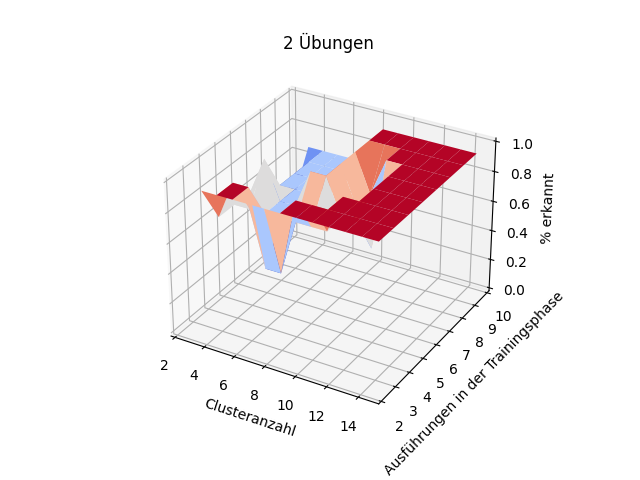
\includegraphics[width=0.7\textwidth]{figures/2_graph.png}
\caption{Bildunterschrift}
\end{figure}
\begin{figure}[h]
\centering
\label{fig:neuron}
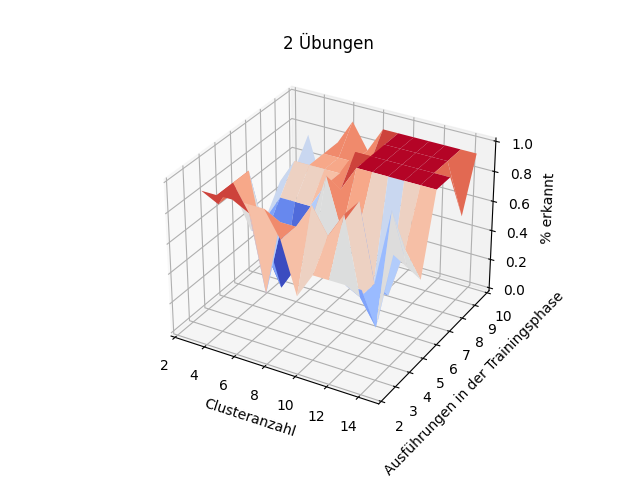
\includegraphics[width=0.7\textwidth]{figures/3_graph.png}
\caption{Bildunterschrift}
\end{figure}
\begin{figure}[h]
\centering
\label{fig:neuron}
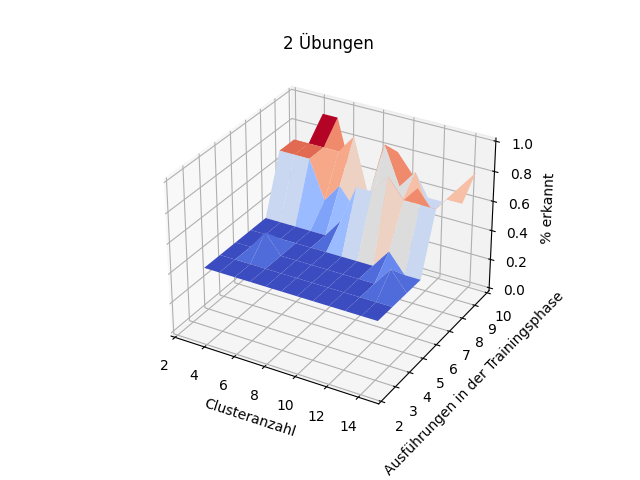
\includegraphics[width=0.7\textwidth]{figures/4_graph.png}
\caption{Bildunterschrift}
\end{figure}
\begin{figure}[h]
\centering
\label{fig:neuron}
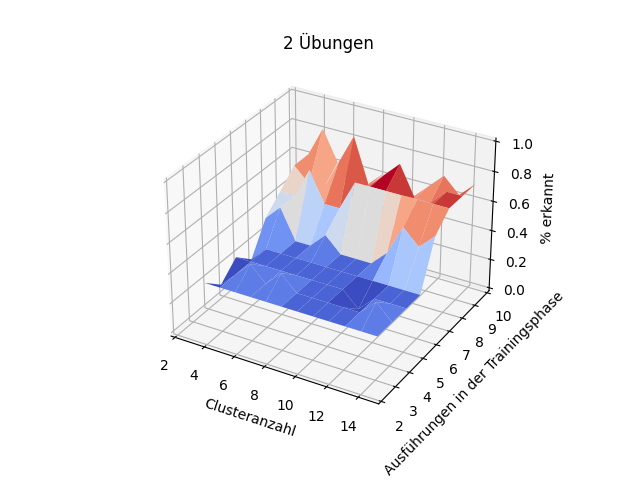
\includegraphics[width=0.7\textwidth]{figures/5_graph.png}
\caption{Bildunterschrift}
\end{figure}




\end{document}
